%%%%%%%%%%%%%%%%%%%%%%%%%%%%%%%%%%%%%%%%%%%%%%%%%%%%%%%%%%%%%%%%%%%%%%%%%%%%%%%%%%
\begin{frame}[fragile]\frametitle{}
\begin{center}
{\Large Notes from Samkhya Darshan}
\end{center}
\end{frame}

%%%%%%%%%%%%%%%%%%%%%%%%%%%%%%%%%%%%%%%%%%%%%%%%%%%%%%%%%%%
\begin{frame}[fragile]\frametitle{भारतीय दर्शन का परिचय}
      \begin{itemize}
	\item भारतीय दर्शन जीवन और ब्रह्मांड के रहस्यों को सुलझाने का अनूठा प्रयास है
	\item दर्शन का अर्थ केवल फिलॉसफी नहीं बल्कि देखना या अनुभव करना भी है
	\item यह वह ज्ञान है जो ऋषियों ने गहरे चिंतन और अनुभव से प्राप्त किया
	\item षड्दर्शन में छ: प्रमुख दर्शन हैं - न्याय, वैशेषिक, सांख्य, योग, मीमांसा और वेदांत
	\item यह सभी वेदों को मानते हैं इसलिए इन्हें आस्तिक दर्शन कहा जाता है
	\item सांख्य दर्शन इन षड्दर्शनों में से एक अत्यंत प्राचीन और प्रभावशाली दर्शन है
	  \end{itemize}
\end{frame}


%%%%%%%%%%%%%%%%%%%%%%%%%%%%%%%%%%%%%%%%%%%%%%%%%%%%%%%%%%%
\begin{frame}[fragile]\frametitle{सांख्य दर्शन का महत्व}
      \begin{itemize}
	\item सांख्य दर्शन को भारतीय चिंतन का आधार स्तंभ माना जाता है
	\item इसके सिद्धांतों का प्रभाव योग, वेदांत, आयुर्वेद और भगवत गीता में भी दिखाई देता है
	\item यह सिखाता है कि यह दुनिया कैसे बनी और हम कौन हैं
	\item हमें दुख क्यों होता है और इससे हमेशा के लिए छुटकारा कैसे मिले
	\item सृष्टि और चेतना के रहस्य को दो मूल तत्वों - पुरुष और प्रकृति के माध्यम से समझाता है
	\item यह रहस्यमई और ज्ञानवर्धक दुनिया में गोता लगाने का अवसर प्रदान करता है
	  \end{itemize}
\end{frame}

%%%%%%%%%%%%%%%%%%%%%%%%%%%%%%%%%%%%%%%%%%%%%%%%%%%%%%%%%%%
\begin{frame}[fragile]\frametitle{सांख्य शब्द का अर्थ}
      \begin{itemize}
	\item सांख्य शब्द संख्या से बना है जिसका अर्थ है गिनती या गणना करना
	\item यह सृष्टि के मूल तत्वों की सटीक गणना करता है
	\item तत्वों के विश्लेषण के आधार पर ज्ञान प्राप्त करने पर जोर देता है
	\item सही ज्ञान (सम्यक ख्याति) तत्वों की सही गिनती और उनके स्वरूप को समझने से मिलता है
	\item दूसरा अर्थ विवेकपूर्ण ज्ञान भी है
	\item हमें सत्य और असत्य, आत्मा और अनात्मा के बीच भेद करना सिखाता है
	  \end{itemize}
\end{frame}

%%%%%%%%%%%%%%%%%%%%%%%%%%%%%%%%%%%%%%%%%%%%%%%%%%%%%%%%%%%%%%%%%%%%%%%%%%%%%%%%%%
\begin{frame}[fragile]\frametitle{Background}

      \begin{itemize}
        \item मनुष्य की हमेशा से जिज्ञासा रही है की हमारा अस्तित्व आया कहां से? हमारे अतीत का कारण क्या है? ब्रह्मांड की उत्पत्ति हुई कहां से? जो हमारी ऋषि मुनि हुए उनको भी यह सब समझना था 
		\item  ढेर सारे मजहब बताते हैं की सृष्टि को किसी ईश्वर ने बना दिया है. इस धार्मिक विचार से हटकर हमारे ऋषि मुनियों ने दी  और जो बहुत तार्किक को शास्त्रीय हो, वो है, सांख्य दर्शन 
		\item सनातन धर्म के केंद्र में जो चार वेद है ऋग्वेद यजुर्वेद सामवेद अथर्ववेद और उनके भाग, आरण्यक, ब्राह्मण , संहिता ,  उपनिषद.  इनके आधार पर जब ऋषि मुनियों ने अध्ययन किया तो छह दर्शन मानव जीवन को समझने के लिए दिये, उसमेसे एक है सांख्य दर्शन 
		\item इनमें किसी में कर्म को ऊपर रखा गया है किसी में भक्ति के ऊपर रखा गया है किसी में ज्ञान को ऊपर रखा गया क्योंकि यही तीन
माध्यम है जो सनातन धर्म में ईश्वर को ईश्वर तक पहुंचने के लिए बताए गए हैं की कर्म ज्ञान और भक्ति तीन तरह के रास्ते हैं.
		\item यह एक दूसरे से काफी अलग है इनमें से कुछ दर्शन बहुईश्वरवाद को मानती हैं कुछ एक भगवान को मानते हैं, और कुछ
भगवान को मानती नहीं है 
\item यह संख्या दर्शन है वह भी अनीश्वरवादी  (agnostic) है वह ईश्वर को भले  न नाकारती हो लेकिन यह भी नहीं मानती ईश्वर सृष्टि की रचना किए होंगे कोई मतलब ऐसे बाहर से कुछ धक्का  दे के  ब्रह्मांड बना हो
      \end{itemize}
\end{frame}


%%%%%%%%%%%%%%%%%%%%%%%%%%%%%%%%%%%%%%%%%%%%%%%%%%%%%%%%%%%%%%%%%%%%%%%%%%%%%%%%%%
\begin{frame}[fragile]\frametitle{सांख्य दर्शन की भूमिका (Introduction to Sāṅkhya Darśana)}
\begin{columns}
    \begin{column}[T]{0.6\linewidth}
      \begin{itemize}
        \item "सांख्य" का अर्थ – क्रमबद्ध विवेचन (rational enumeration), तार्किक, विश्लेषणात्मक और वैज्ञानिक दृष्टिकोण
        \item दर्शन is a proposed mental model to explain the origin of the universe as well as how it runs!!		
        \item कपिल मुनि (Kapila Muni)   प्रवर्तक , 700 BC
        \item \textbf{अनीश्वरवादी} (Anīśvaravādī, Agnostic), ईश्वर को सृष्टिकर्ता नहीं मानता
        \item फिर भी यह \textbf{आस्तिक} (Āstika) दर्शन है,  वेदों को प्रमाण मानता है
        \item गीता, भागवत, महाभारत में इसके तत्वों का उल्लेख
        \item बौद्ध (नास्तिक) और आस्तिक परंपराओं दोनों पर इसका प्रभाव
		\item बुद्ध ने अपना बचपन कपिलवस्तु नाम की नगरी पर उन्होंने बिताया है 

      \end{itemize}
    \end{column}
    \begin{column}[T]{0.4\linewidth}
      \begin{center}
        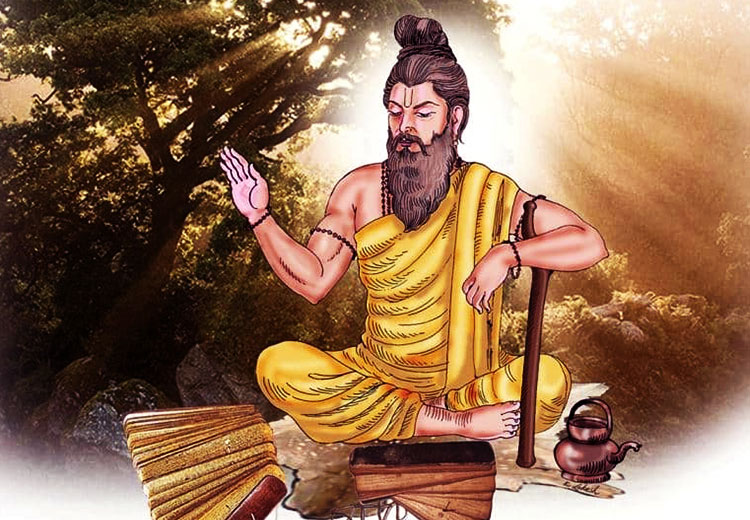
\includegraphics[width=\linewidth,keepaspectratio]{sankhya1}
		
        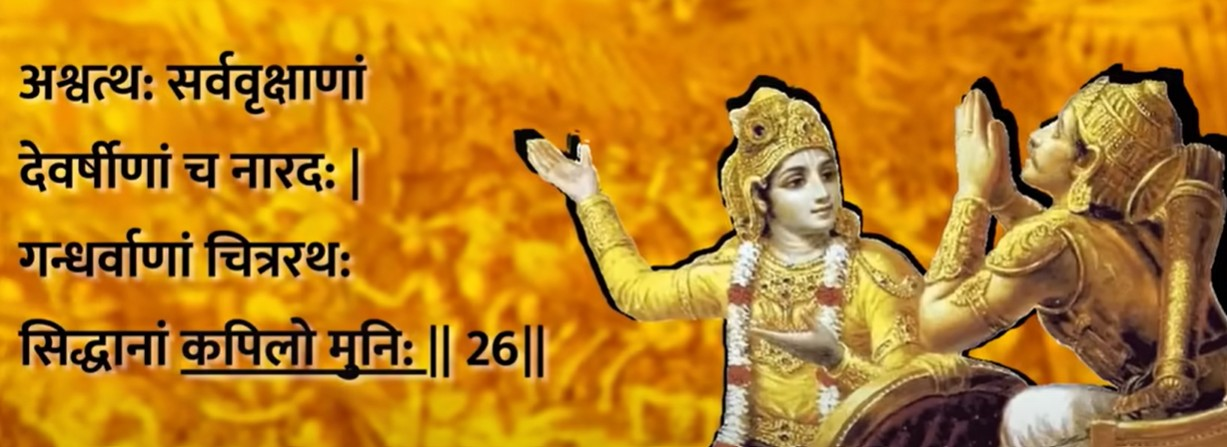
\includegraphics[width=\linewidth,keepaspectratio]{sankhya2}
		
		{\tiny (Ref: Samkhya Darshan - HyperQuest)}
		
      \end{center}	
    \end{column}
\end{columns}
\end{frame}


%%%%%%%%%%%%%%%%%%%%%%%%%%%%%%%%%%%%%%%%%%%%%%%%%%%%%%%%%%%
\begin{frame}[fragile]\frametitle{महर्षि कपिल और सांख्य सूत्र}
      \begin{itemize}
	\item परंपरागत रूप से सांख्य दर्शन के प्रणेता महर्षि कपिल माने जाते हैं
	\item उन्हें अत्यंत प्राचीन और सिद्ध ऋषि माना जाता है
	\item उनका मुख्य ग्रंथ सांख्य सूत्र माना जाता है
	\item कुछ विद्वान सांख्यकारिका को सबसे प्रामाणिक ग्रंथ मानते हैं
	\item सांख्यकारिका को ईश्वर कृष्ण ने लिखा है
	\item यह सांख्य का सबसे प्राचीन उपलब्ध ग्रंथ माना जाता है
	  \end{itemize}
\end{frame}

%%%%%%%%%%%%%%%%%%%%%%%%%%%%%%%%%%%%%%%%%%%%%%%%%%%%%%%%%%%%%%%%%%%%%%%%%%%%%%%%%%
\begin{frame}[fragile]\frametitle{मुख्य ग्रंथ (Principal Texts)}
\begin{columns}
    \begin{column}[T]{0.6\linewidth}
      \begin{itemize}
        \item मूल ग्रंथ: \textbf{सांख्य प्रवचन सूत्र (Sāṅkhya Pravacana Sūtra)} कपिल मुनि द्वारा रचित, वो ग्रंथ आज अपने मूल रूप में मिलता ही नहीं है
        \item वर्तमान में प्रमुख ग्रंथ: \textbf{सांख्य कारिका (Sāṅkhya Kārikā)} रचयिता: ईश्वरकृष्ण (Īśvarakṛṣṇa), लगभग 300 ई.पू.
        \item 72 सूत्रों में दर्शन की पूर्ण प्रस्तुति
        \item कारिका पर अनेक टीकाएँ : गौड़पाद, वाचस्पति मिश्र आदि द्वारा
        \item परंपरा में मौखिक ज्ञान से लिखित परंपरा का स्थानांतरण
      \end{itemize}
    \end{column}
    \begin{column}[T]{0.4\linewidth}
      \begin{center}
        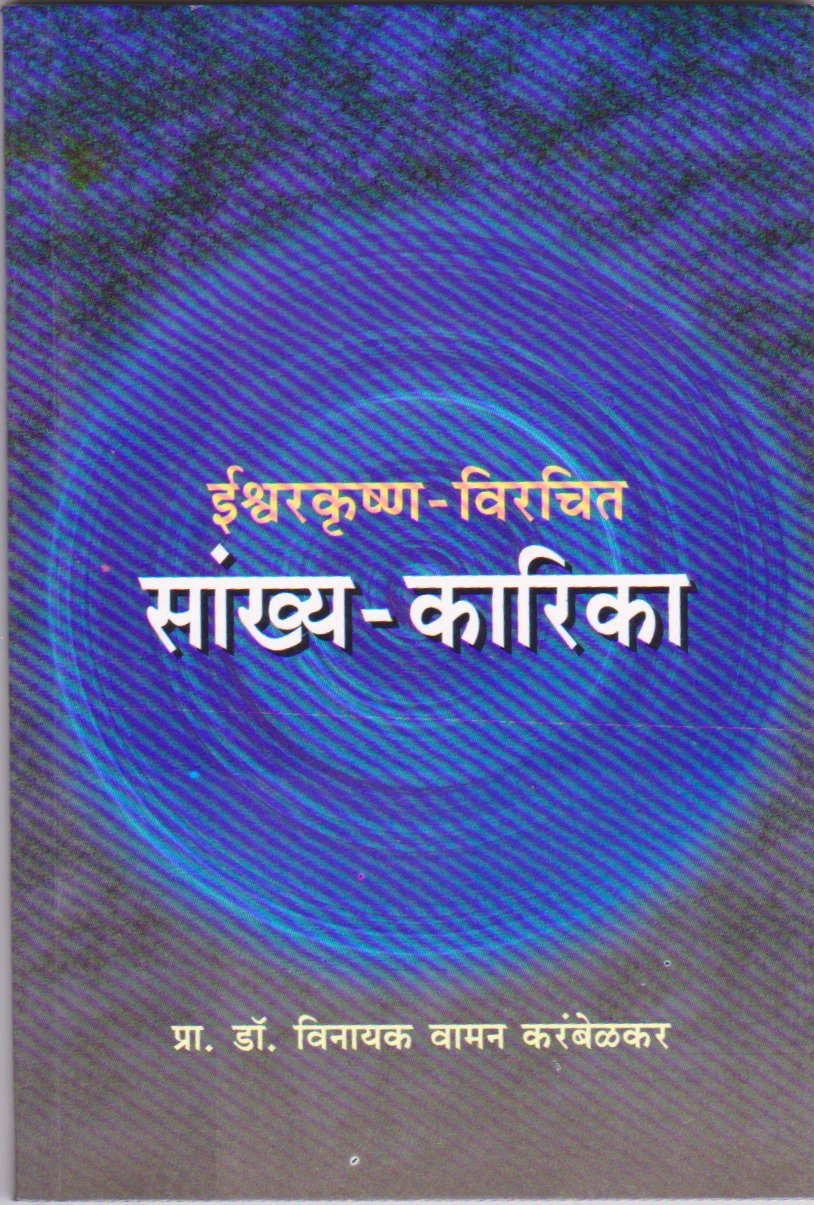
\includegraphics[width=\linewidth,keepaspectratio]{sankhya3}
      \end{center}	
    \end{column}
\end{columns}
\end{frame}

%%%%%%%%%%%%%%%%%%%%%%%%%%%%%%%%%%%%%%%%%%%%%%%%%%%%%%%%%%%%%%%%%%%%%%%%%%%%%%%%%%
\begin{frame}[fragile]\frametitle{सत्कार्यवाद (Satkāryavāda)}
\begin{columns}
    \begin{column}[T]{0.6\linewidth}
      \begin{itemize}
		\item सत कर्म से ही सत कार्य उत्पन्न होते हैं ऐसा नहीं की असत से सत नहीं बन सकता है 
		\item आप यह नहीं का सकते की कुछ नहीं था और उससे कुछ बन गया
        \item कारण (cause) में कार्य (effect) की पूर्वस्थिति होती है. For effect there has to be a cause.
        \item \textbf{सत् (Sat)} से ही \textbf{सत्कार्य (Satkārya)} उत्पन्न होता है
        \item "शून्य से कुछ नहीं बनता" — \textbf{असत्कार्यवाद} का खंडन
        \item उदाहरण: बीज में वृक्ष की संभावना
        \item कार्य, कारण का दृश्य रूप है, कारण can be invisible, say, a thought.
        \item कारण के दो प्रकार: \textbf{निमित्त} (Nimitta) और \textbf{उपादान} (Upādāna)

      \end{itemize}
    \end{column}
    \begin{column}[T]{0.4\linewidth}
      \begin{center}
        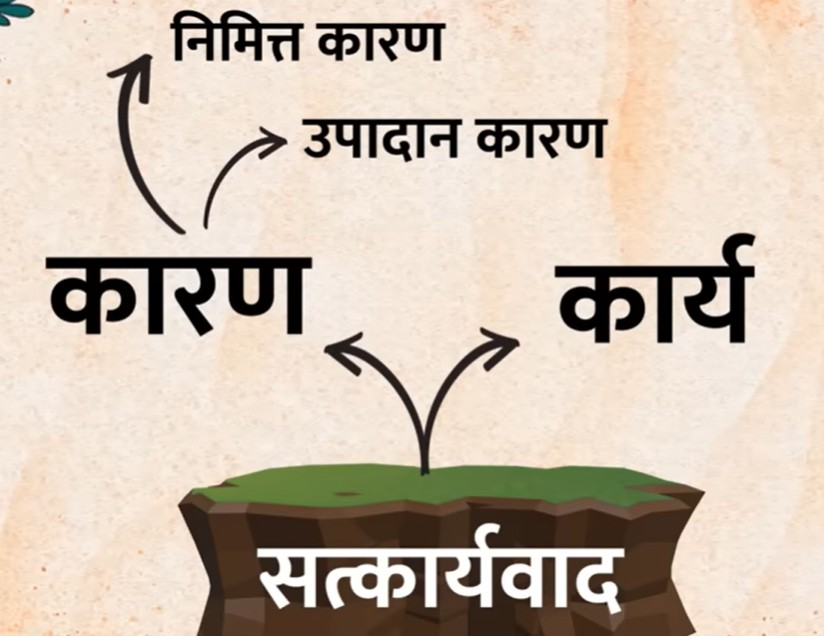
\includegraphics[width=\linewidth,keepaspectratio]{sankhya4}
		
		घड़े के लिए मिट्टी उपादान, कुम्हार निमित्त
		
        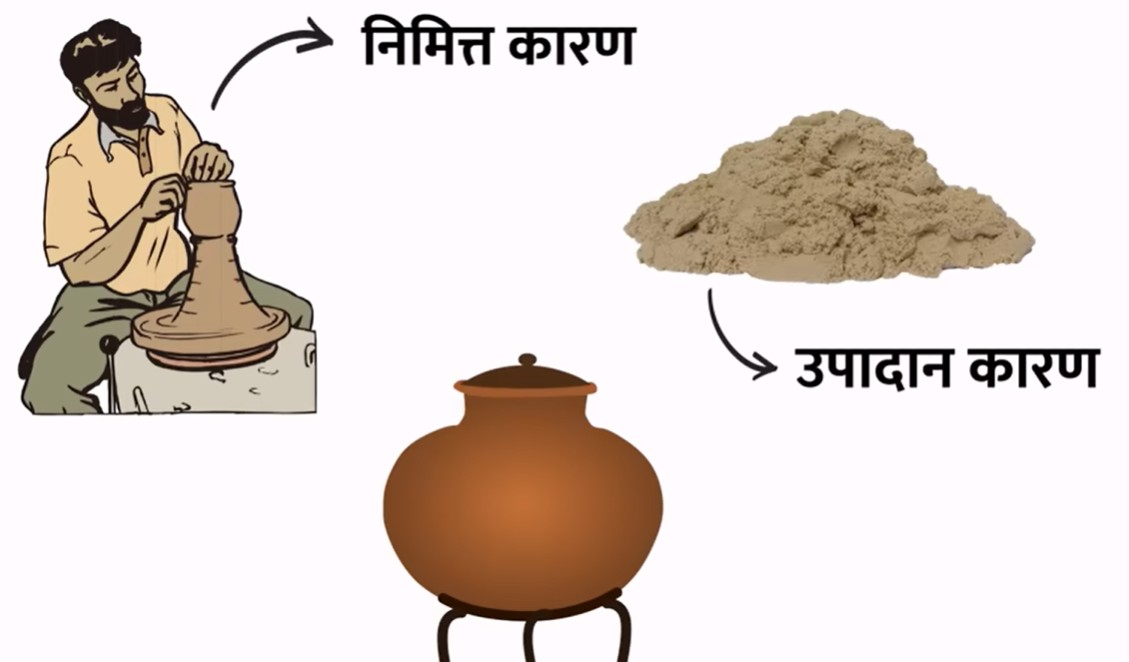
\includegraphics[width=\linewidth,keepaspectratio]{sankhya5}
		
		{\tiny (Ref: Samkhya Darshan - HyperQuest)}
		
      \end{center}	
    \end{column}
\end{columns}
\end{frame}

%%%%%%%%%%%%%%%%%%%%%%%%%%%%%%%%%%%%%%%%%%%%%%%%%%%%%%%%%%%
\begin{frame}[fragile]\frametitle{सत्कार्यवाद का सिद्धांत}
      \begin{itemize}
	\item सांख्य का अत्यंत महत्वपूर्ण दार्शनिक सिद्धांत है सत्कार्यवाद
	\item कार्य (इफेक्ट) अपनी उत्पत्ति से पहले ही अपने कारण में अव्यक्त रूप में मौजूद रहता है
	\item सृष्टि में कुछ भी बिल्कुल नया उत्पन्न नहीं होता
	\item जो पहले से ही कारण में बीज रूप में विद्यमान था, वही प्रकट हो जाता है
	\item उदाहरण: दही बनने से पहले वह दूध में ही अव्यक्त रूप से मौजूद होता है
	\item तिल में तेल पहले से ही विद्यमान होता है, उसे केवल निकालकर प्रकट किया जाता है
	  \end{itemize}
\end{frame}

%%%%%%%%%%%%%%%%%%%%%%%%%%%%%%%%%%%%%%%%%%%%%%%%%%%%%%%%%%%
\begin{frame}[fragile]\frametitle{सत्कार्यवाद के उदाहरण}
      \begin{itemize}
	\item दूध ही दही में परिवर्तित होता है, पानी से दही नहीं बन सकता
	\item रेत से तेल नहीं निकाला जा सकता क्योंकि वह उसमें मौजूद नहीं है
	\item मिट्टी में घड़ा बनने की क्षमता निहित होती है, इसलिए कुम्हार मिट्टी से घड़ा बना पाता है
	\item हवा से घड़ा नहीं बन सकता क्योंकि उसमें यह क्षमता नहीं है
	\item यह संपूर्ण व्यक्त सृष्टि अपनी उत्पत्ति से पहले मूल प्रकृति में अव्यक्त रूप से मौजूद थी
	\item प्रकृति ही इस संपूर्ण भौतिक जगत का एकमात्र उपादान कारण (मटेरियल कॉज) है
	  \end{itemize}
\end{frame}

%%%%%%%%%%%%%%%%%%%%%%%%%%%%%%%%%%%%%%%%%%%%%%%%%%%%%%%%%%%
\begin{frame}[fragile]\frametitle{सृष्टि की उत्पत्ति: पुरुष और प्रकृति का सानिध्य}
      \begin{itemize}
	\item सृष्टि की प्रक्रिया तब आरंभ होती है जब पुरुष और प्रकृति का सानिध्य होता है
	\item यह कोई भौतिक संपर्क या मिलन नहीं है बल्कि एक प्रकार की निकटता या प्रभाव है
	\item उदाहरण: चुंबक स्वयं निष्क्रिय होते हुए भी अपनी निकटता से लोहे में गति उत्पन्न करता है
	\item राजा की उपस्थिति मात्र से मंत्री और कर्मचारी सक्रिय होकर अपने कार्य करने लगते हैं
	\item चेतन पुरुष के सानिध्य मात्र से अचेतन प्रकृति में हलचल शुरू हो जाती है
	\item इससे प्रकृति के तीनों गुणों की साम्यावस्था भंग हो जाती है और विक्षोभ उत्पन्न होता है
	  \end{itemize}
\end{frame}

%%%%%%%%%%%%%%%%%%%%%%%%%%%%%%%%%%%%%%%%%%%%%%%%%%%%%%%%%%%
\begin{frame}[fragile]\frametitle{सृष्टि विकास की शुरुआत}
      \begin{itemize}
	\item पुरुष के सानिध्य से रजोगुण जो क्रिया का प्रतीक है, सक्रिय हो उठता है
	\item सत्व तथा तमस गुणों में भी गति आ जाती है
	\item यहीं से सृष्टि का विकास क्रम जिसे तत्व परिणाम कहा जाता है, शुरू होता है
	\item प्रकृति से बुद्धि, महत्व, अहंकार, मन, ज्ञानेंद्रियां, कर्मेंद्रियां बनते हैं
	\item तन्मात्राएं और पंचमहाभूत का विकास होता है
	\item यह विकास क्रम अत्यंत रोचक है और हमारे अस्तित्व की संरचना को समझने में मदद करता है
	  \end{itemize}
\end{frame}

%%%%%%%%%%%%%%%%%%%%%%%%%%%%%%%%%%%%%%%%%%%%%%%%%%%%%%%%%%%%%%%%%%%%%%%%%%%%%%%%%%
\begin{frame}[fragile]\frametitle{ब्रह्मांड}

      \begin{itemize}
		\item ईश्वर (निमित्त) ने ब्रह्मांड को बनाया है लेकिन उपादान कारण क्या है? मिट्टी कहां से आई जो घड़ा बना उसके लिए ? 
		\item भगवान हो या ना हो लेकिन उपादान कारण तो चाहिए तो इसलिए उपादान कारण को फिर खोजना है. 
		\item हमारे पास कार्य हो कारण पता ही ना हो जैसे ये ब्रह्मांड कार्य तो हमें पता है की ब्रह्मांड बन गया है लेकिन कारण नहीं पता. संख्या दर्शन ये बोलता है की अगर हमारे पास कार्य है तो कार्य को देख कर कारण का अनुमान लगाया जा सकता है 
		\item जैसे की बच्चेको देखकर उसकेमातापिता कैसे होंगे यह अनुमान लगाया जा सकता है. या फिर ढेर सारे जोडे को खड़ा कर दिया जाए तो कुछ हद तक यह बताया जा सकता है की वो किसका बेटा है 
      \end{itemize}


\end{frame}

%%%%%%%%%%%%%%%%%%%%%%%%%%%%%%%%%%%%%%%%%%%%%%%%%%%%%%%%%%%%%%%%%%%%%%%%%%%%%%%%%%
\begin{frame}[fragile]\frametitle{ब्रह्मांड}

      \begin{itemize}
		\item आपके पास घडा है और आपके हाथ में बहुत ढेर सारे अलग-अलग तरह के पदार्थ दे दिए जाए तो आप ये तो नहीं बोलोगे की यह धर्म मोम का बना होगा मिट्टी जैसा रेट जैसा कुछ दिखेगा तो आप उसको बता सकते हो.
		\item ``ब्रह्मांड हमारे पास है है तो इसका कारण भी ब्रह्मांड जैसा होना चाहिए ''
      \end{itemize}

      \begin{center}
	
        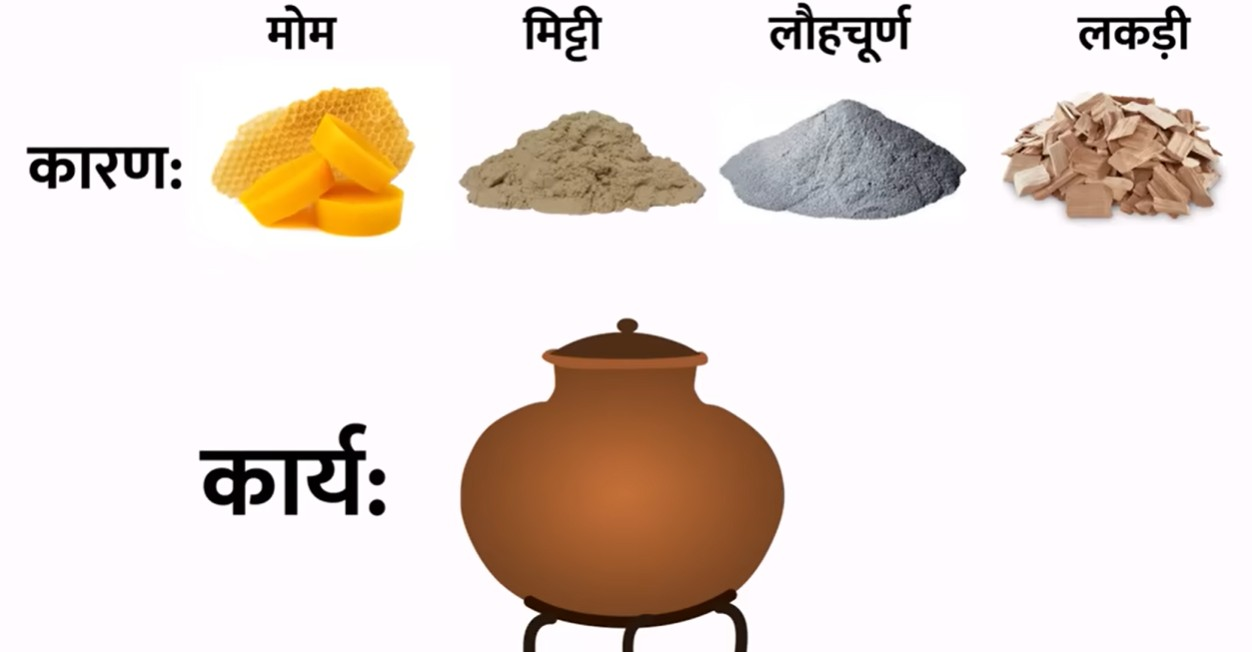
\includegraphics[width=0.8\linewidth,keepaspectratio]{sankhya6}
		
		{\tiny (Ref: Samkhya Darshan - HyperQuest)}
		
      \end{center}	
\end{frame}


%%%%%%%%%%%%%%%%%%%%%%%%%%%%%%%%%%%%%%%%%%%%%%%%%%%%%%%%%%%%%%%%%%%%%%%%%%%%%%%%%%
\begin{frame}[fragile]\frametitle{ब्रह्मांड}

      \begin{itemize}
		\item  ब्रह्मांड में तीन चीज प्रमुखता से दिखती 
		\item बहुत सी चीज प्रकाश वहां है प्रकाशित हैं बहुत तेजस्वी हैं और बहुत ढेर सारी चीज गतिमान है और तीसरी चीज की बहुत सी चीज
अंधेरे में है तो ये तीन तरह के उनको निरीक्षण दिखते हैं ब्रह्मांड में 
		\item पृथ्वी पर भी निरीक्षण करते हैं तो कुछ इंसान जो है बहुत सुखी दिखते हैं उनके चेहरे पे तेज दिखता है कुछ इंसान भागदौड़ी में है लेकिन बहुत पेन में है पीड़ा में है दुखी हैं और कुछ इंसान एकदम ही आलसी हैं मतलब उदासीन है जैसे लगता है जीवन में फंसे हुए हैं 
		\item तो ये तीन तरह की चीज ब्रह्मांड में हमारे ऋषि मुनियों को दिखी तो उन्होंने ये माना की जब ब्रह्मांड में कार्य में ये तीन इफेक्ट है यह तीन तरह के गुण है तो उसके कारण में भी ये तीन गुण होने चाहिए तभी उससे ये ब्रह्मांड आ  सकता है अगर कारण में तीन गुण नहीं है तो कार्य
में भी ये तीन गुण नहीं होंगे 
		\item सांख्य दर्शन ने ब्रह्मांड का जो उपादान कारण है उसको प्रकृति माना
		\item प्रकृति मतलब प्र+कृति, कृति मतलब कार्य,  प्रा-> पहले. तो कार्य से पहले जो कारण आया है ब्रह्मांड का उसको प्रकृति
बोला
      \end{itemize}

\end{frame}

%%%%%%%%%%%%%%%%%%%%%%%%%%%%%%%%%%%%%%%%%%%%%%%%%%%%%%%%%%%
\begin{frame}[fragile]\frametitle{सांख्य दर्शन का द्वैतवाद}
      \begin{itemize}
	\item सांख्य दर्शन की सबसे बड़ी विशेषता इसका द्वैतवाद है
	\item द्वैतवाद का अर्थ: सृष्टि के मूल में दो स्वतंत्र, अनादि और अनंत सत्ताएं हैं
	\item पहली सत्ता: पुरुष - चेतना, आत्मा या ज्ञाता
	\item दूसरी सत्ता: प्रकृति - जड़ पदार्थ, ऊर्जा या अचेतन मूल तत्व
	\item यह दोनों एक दूसरे से बिल्कुल भिन्न हैं
	\item सृष्टि की प्रक्रिया इन दोनों के संयोग (सानिध्य या निकटता) से शुरू होती है
	  \end{itemize}
\end{frame}


%%%%%%%%%%%%%%%%%%%%%%%%%%%%%%%%%%%%%%%%%%%%%%%%%%%%%%%%%%%
\begin{frame}[fragile]\frametitle{पुरुष: चेतना का सिद्धांत}
      \begin{itemize}
	\item पुरुष का स्वभाव ही चेतन है - वह जानने वाला, देखने वाला (दृष्टा) और अनुभव करने वाला (भोक्ता) है
	\item दुनिया में जो कुछ भी जानने, देखने या अनुभव करने की क्षमता है वह पुरुष के कारण ही है
	\item यद्यपि वह ज्ञाता और भोक्ता है, वह स्वयं निष्क्रिय (अकर्ता) है
	\item केवल एक साक्षी (विटनेस) की तरह प्रकृति के खेल को देखता है
	\item वह निर्लेप है - किसी वस्तु या अनुभव से लिप्त नहीं होता
	\item सुख-दुख, पाप-पुण्य, जन्म-मरण से परे है - यह सब प्रकृति के विकार हैं
	  \end{itemize}
\end{frame}

%%%%%%%%%%%%%%%%%%%%%%%%%%%%%%%%%%%%%%%%%%%%%%%%%%%%%%%%%%%
\begin{frame}[fragile]\frametitle{पुरुष की विशेषताएं}
      \begin{itemize}
	\item पुरुष में कोई परिवर्तन नहीं होता - वह निर्विकार है, हमेशा एक जैसा रहता है
	\item जन्म, वृद्धि, क्षय, मृत्यु - यह सब प्रकृति के धर्म हैं, पुरुष के नहीं
	\item सांख्य की महत्वपूर्ण मान्यता: पुरुष अनेक हैं
	\item हर जीव में एक अलग पुरुष (चेतना) वास करती है
	\item इसीलिए हर जीव का अनुभव (सुख-दुख, जन्म-मरण, मोक्ष) अलग-अलग होता है
	\item अगर पुरुष एक होता तो एक के मुक्त होने पर सभी मुक्त हो जाते
	  \end{itemize}
\end{frame}

%%%%%%%%%%%%%%%%%%%%%%%%%%%%%%%%%%%%%%%%%%%%%%%%%%%%%%%%%%%
\begin{frame}[fragile]\frametitle{पुरुष के अस्तित्व के तर्क}
      \begin{itemize}
	\item पहला तर्क: जड़ वस्तुएं (कुर्सी, मेज) किसी चेतन भोक्ता के उपयोग के लिए होती हैं
	\item सारी सृष्टि जो जड़ प्रकृति से बनी है, किसी चेतन पुरुष के भोग और मोक्ष के लिए है
	\item दूसरा तर्क: हर किसी के मन में मोक्ष या दुख से मुक्ति की स्वाभाविक इच्छा होती है
	\item यह इच्छा तभी सार्थक हो सकती है जब कोई बंधन में हो और मुक्त होने की क्षमता रखता हो
	\item तीसरा तर्क: प्रकृति के तीन गुण (सत्व, रजस, तमस) स्वयं अचेतन हैं
	\item उन्हें अनुभव करने वाला कोई चेतन तत्व अवश्य होना चाहिए - वही पुरुष है
	  \end{itemize}
\end{frame}

%%%%%%%%%%%%%%%%%%%%%%%%%%%%%%%%%%%%%%%%%%%%%%%%%%%%%%%%%%%
\begin{frame}[fragile]\frametitle{प्रकृति: जड़ जगत का मूल कारण}
      \begin{itemize}
	\item प्रकृति अपने स्वभाव से अचेतन है - उसमें अपनी कोई चेतना नहीं होती
	\item वह स्वयं न तो जान सकती है न ही अनुभव कर सकती है
	\item इसके विपरीत प्रकृति अत्यंत सक्रिय है - वही सृष्टि की रचना करने वाली शक्ति है
	\item सारा बदलाव, सारी गति, सारा कार्य प्रकृति में ही संभव होता है
	\item जहां पुरुष अनेक माने गए हैं, वहीं प्रकृति केवल एक ही है
	\item उसी एक मूल प्रकृति से यह विविधताओं से भरा ब्रह्मांड उत्पन्न होता है
	  \end{itemize}
\end{frame}

%%%%%%%%%%%%%%%%%%%%%%%%%%%%%%%%%%%%%%%%%%%%%%%%%%%%%%%%%%%
\begin{frame}[fragile]\frametitle{प्रकृति के नाम और स्वरूप}
      \begin{itemize}
	\item प्रकृति को प्रधान भी कहा जाता है क्योंकि वही सभी कार्यों का मूल कारण है
	\item उसे अव्यक्त भी कहते हैं क्योंकि अपनी मूल अवस्था में वह प्रकट नहीं होती
	\item हमारी इंद्रियों द्वारा सीधे जानी नहीं जा सकती
	\item प्रकृति की सबसे महत्वपूर्ण विशेषता: वह त्रिगुणात्मिका है
	\item यानी तीन गुणों या शक्तियों से बनी है
	\item यह तीन गुण हैं: सत्व, रजस और तमस
	  \end{itemize}
\end{frame}


%%%%%%%%%%%%%%%%%%%%%%%%%%%%%%%%%%%%%%%%%%%%%%%%%%%%%%%%%%%%%%%%%%%%%%%%%%%%%%%%%%
\begin{frame}[fragile]\frametitle{प्रकृति – उपादान कारण (Prakṛti as Material Cause)}

      \begin{itemize}
        \item ब्रह्मांड का उपादान कारण: \textbf{प्रकृति (Prakṛti)},         प्रकृति = \textbf{प्रधान} = मूल कार्य (ब्रह्मांड) का स्रोत. \textbf{अव्यक्त} (Avyakta), \textbf{अज} (Unborn), \textbf{अनादि} (Eternal)
        \item प्रकृति त्रिगुणात्मक: \textbf{सत्त्व}, \textbf{रजस्}, \textbf{तमस्}, सत्त्व – प्रकाश, रजस् – गति, तमस् – आलस 
		\item प्रकृति तो बहुत असीम माना गया है लेकिन असीम मरने के साथ-साथ उसको जड़ माना गया की उसमें बुद्धि नहीं है वो खुद से नहीं बना सकती 
		\item कौन से गुण किस अनुपात में मिल के सत रज  तम का कौन-कौन सा किस अनुपात से मिलकर यह ब्रह्मांड बने गए
ब्रह्मांड की कौन सी चीज कितने अनुपात में बनेगी ये प्रकृति के बस का नहीं है क्योंकि उसके पास खुद की चेतना नहीं है वो जड़ है 
        \item प्रकृति जड़ (बुद्धिहीन ) है, चेतना नहीं रखती. मूल प्रकृति बस आइडिया है वह अव्यक्त है 
        \item जब साम्यावस्था भंग होती है, तभी सृष्टि प्रारंभ
		\item सांख्य दर्शन बोलता है पुरुष जो ये चेतना है  
	
      \end{itemize}

\end{frame}

%%%%%%%%%%%%%%%%%%%%%%%%%%%%%%%%%%%%%%%%%%%%%%%%%%%%%%%%%%%
\begin{frame}[fragile]\frametitle{प्रकृति के तीन गुण: सत्व, रजस और तमस}
      \begin{itemize}
	\item सत्वगुण: प्रकाश, ज्ञान, सुख, शांति, हल्कापन और अच्छाई का प्रतीक
	\item मन में स्थिरता, निर्मलता और प्रसन्नता लाता है, प्रतीकात्मक रंग सफेद
	\item रजसगुण: क्रिया, गति, बेचैनी, इच्छा, दुख और ऊर्जा का प्रतिनिधित्व
	\item हमें कर्म करने के लिए प्रेरित करता है लेकिन अशांति का कारण भी बनता है, रंग लाल
	\item तमसगुण: अंधकार, अज्ञान, आलस्य, मोह और भारीपन का द्योतक
	\item ज्ञान को ढकता है और हमें निष्क्रिय बनाता है, प्रतीकात्मक रंग काला
	  \end{itemize}
\end{frame}

%%%%%%%%%%%%%%%%%%%%%%%%%%%%%%%%%%%%%%%%%%%%%%%%%%%%%%%%%%%
\begin{frame}[fragile]\frametitle{त्रिगुण की कार्यप्रणाली}
      \begin{itemize}
	\item यह तीनों गुण हमेशा एक साथ रहते हैं जैसे एक रस्सी के तीन धागे आपस में गूंथे होते हैं
	\item कभी भी एक दूसरे से पूरी तरह अलग नहीं होते
	\item हालांकि उनकी प्रबलता बदलती रहती है - कभी सत्व, कभी रजस, कभी तमस अधिक प्रभावी
	\item इन्हीं गुणों के विभिन्न अनुपातों में मिलने से दुनिया की सारी विविधता पैदा होती है
	\item जब सृष्टि नहीं होती (प्रलय की अवस्था) तब तीनों गुण पूर्ण साम्य अवस्था में रहते हैं
	\item सृष्टि की प्रक्रिया तब शुरू होती है जब पुरुष के सानिध्य से इस संतुलन में विक्षोभ उत्पन्न होता है
	  \end{itemize}
\end{frame}

%%%%%%%%%%%%%%%%%%%%%%%%%%%%%%%%%%%%%%%%%%%%%%%%%%%%%%%%%%%
\begin{frame}[fragile]\frametitle{प्रकृति के अस्तित्व के तर्क}
      \begin{itemize}
	\item पहला तर्क: दुनिया की सभी वस्तुएं सीमित हैं, एक दूसरे पर निर्भर हैं
	\item इन सभी सीमित वस्तुओं का कोई मूल असीम, स्वतंत्र और अनाश्रित कारण होना चाहिए - वही प्रकृति है
	\item दूसरा तर्क: दुनिया की सभी वस्तुओं में त्रिगुणात्मकता के लक्षण दिखते हैं
	\item वे सुख, दुख या मोह उत्पन्न करती हैं - यह साबित करता है कि उनका मूल कारण भी त्रिगुणात्मक है
	\item तीसरा तर्क: कार्य-कारण का नियम - हर कार्य का कोई न कोई कारण अवश्य होता है
	\item यह व्यक्त जगत एक कार्य है, इसलिए इसका कोई अव्यक्त कारण होना चाहिए - वही प्रकृति है
	  \end{itemize}
\end{frame}

%%%%%%%%%%%%%%%%%%%%%%%%%%%%%%%%%%%%%%%%%%%%%%%%%%%%%%%%%%%%%%%%%%%%%%%%%%%%%%%%%%
\begin{frame}[fragile]\frametitle{पुरुष – चेतन तत्त्व (Puruṣa – Conscious Principle)}
सांख्य दर्शन को द्वैतवाद बोलते हैं की दो प्रमुख मूल तत्व हैं एक है प्रकृति जो कारण है उपादान कारण है जिससे ब्रह्मांड बना है और फिर उसे
प्रकृति में चूंकि जड़ता है उसके पास खुद का दिमाग नहीं है वो बस साम्यावस्था में है उसके पास तीन गुण इसलिए हैं क्योंकि ब्रह्मांड में भी तीन गुण देखते हैं यह तीन गुण कैसे मिलके ब्रह्मांड बनेगा इसके लिए चाहिए चेतना और उसे चेतना को फिर पुरुष बोला अब प्रकृति और पुरुष समीप आते हैं उनसे ब्रह्मांड कैसे बनता है

\begin{columns}
    \begin{column}[T]{0.5\linewidth}
      \begin{itemize}
        \item \textbf{पुरुष (Puruṣa)} – शुद्ध चेतना
        \item अनुभव करने वाला, किन्तु कर्ता नहीं
        \item \textbf{निर्गुण}, \textbf{अक्रिय}, \textbf{साक्षी रूप}
        \item अनेक पुरुष – हर जीव में एक चेतना
        \item प्रकृति और पुरुष के संयोग से सृष्टि आरंभ होती है
        \item पुरुष का उद्देश्य – केवल \textbf{दर्शन} और \textbf{अनुभव}
        \item पुरुष दुख के कारण नहीं, मात्र दर्शक है
      \end{itemize}
    \end{column}
    \begin{column}[T]{0.5\linewidth}
      \begin{center}
        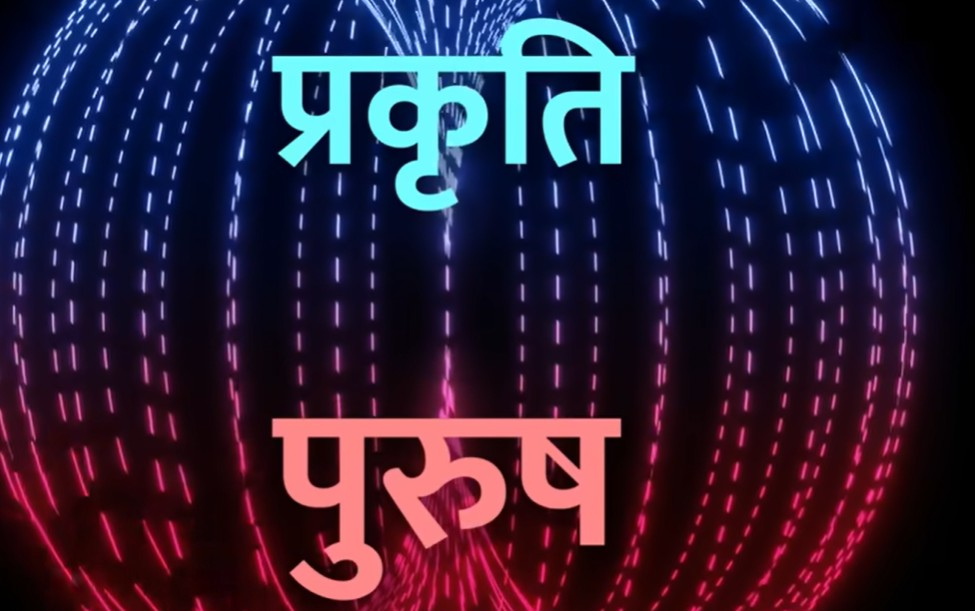
\includegraphics[width=\linewidth,keepaspectratio]{sankhya7}
      \end{center}	
    \end{column}
\end{columns}
\end{frame}

%%%%%%%%%%%%%%%%%%%%%%%%%%%%%%%%%%%%%%%%%%%%%%%%%%%%%%%%%%%
\begin{frame}[fragile]\frametitle{प्रकृति और पुरुष का मूलभूत सिद्धांत}
      \begin{itemize}
          \item ब्रह्मांड का मूल कारण प्रकृति है और ब्रह्मांड स्वयं कार्य है
          \item कारण तब कहलाता है जब उसमें पोटेंशियल हो और वह कार्य में बदल सके
          \item जैसे बीज से पेड़ उगता है - बीज कारण है, पेड़ कार्य है
          \item कारण बनने के लिए पोटेंशियल का रिलीज़ होना अत्यंत महत्वपूर्ण है
          \item प्रकृति को उपादान कारण कहा गया है क्योंकि वह ब्रह्मांड में परिवर्तित होती है
          \item प्रकृति सदा बेचैन रहती है क्योंकि उसके अंदर असीम पोटेंशियल है
          \item प्रकृति formless और असीम है लेकिन फॉर्म में आने की क्षमता रखती है
      \end{itemize}
\end{frame}

%%%%%%%%%%%%%%%%%%%%%%%%%%%%%%%%%%%%%%%%%%%%%%%%%%%%%%%%%%%
\begin{frame}[fragile]\frametitle{पुरुष की प्रकृति और चेतना}
      \begin{itemize}
          \item पुरुष एक चेतना मात्र है जो निर्गुण है (कोई गुण नहीं)
          \item चेतना का अर्थ है अनुभव करना - यही पुरुष का मूल कार्य है
          \item पुरुष को अपनी चेतना सिद्ध करने के लिए कुछ अनुभव करना पड़ता है
          \item प्रकृति बेचैन है अपनी पोटेंशियल रिलीज़ करने के लिए
          \item पुरुष बेचैन है चेतना बनने और अनुभव करने के लिए
          \item दोनों अपने अस्तित्व को बचाने के लिए एक साथ आते हैं
          \item यह संयोग ब्रह्मांड निर्माण का कारण बनता है
      \end{itemize}
\end{frame}

%%%%%%%%%%%%%%%%%%%%%%%%%%%%%%%%%%%%%%%%%%%%%%%%%%%%%%%%%%%
\begin{frame}[fragile]\frametitle{पुरुष की अनेकता और प्रकृति की एकता}
      \begin{itemize}
          \item पुरुष संख्या में अनेक हैं लेकिन प्रकृति केवल एक है
          \item प्रकृति का आकार अनंत है जबकि पुरुषों की संख्या अनंत है
          \item अलग-अलग जीवात्माओं के अनुभव भिन्न-भिन्न होते हैं
          \item एक ही घटना का अनुभव अलग-अलग प्राणियों के लिए अलग होता है
          \item कुत्ता अपने मालिक को भगवान मानता है, बिल्ली खुद को भगवान मानती है
          \item यह चेतना का अंतर पुरुष की अनेकता को सिद्ध करता है
          \item प्रकृति को मैटर और एनर्जी के रूप में समझा जा सकता है जो असीम है
      \end{itemize}
\end{frame}

%%%%%%%%%%%%%%%%%%%%%%%%%%%%%%%%%%%%%%%%%%%%%%%%%%%%%%%%%%%
\begin{frame}[fragile]\frametitle{पुरुष-प्रकृति संयोग से महत्तत्त्व की उत्पत्ति}
      \begin{itemize}
          \item जब चेतना प्रकृति के समीप आकर अनुभव करना शुरू करती है
          \item सबसे पहले महत्तत्त्व (बुद्धি) की उत्पत्ति होती है
          \item प्रकृति अपने formlessness से चेतना के अनुभव पर पहला तत्व देती है
          \item बुद्धि में निर्णय करने की क्षमता आ जाती है
          \item यह प्रकृति का जाल है चेतना को फंसाने के लिए
          \item बुद्धि मिलने के बाद चेतना दूर नहीं जा सकती
          \item यह प्रकृति का पहला चरण है चेतना को अपने खेल में फंसाने का
      \end{itemize}
\end{frame}

%%%%%%%%%%%%%%%%%%%%%%%%%%%%%%%%%%%%%%%%%%%%%%%%%%%%%%%%%%%
\begin{frame}[fragile]\frametitle{अहंकार तत्त्व की उत्पत्ति और व्यक्तित्व निर्माण}
      \begin{itemize}
          \item बुद्धि के बाद प्रकृति द्वितीय तत्व अहंकार देती है
          \item अहंकार के आते ही व्यक्तिगत पहचान बनती है (जैसे विशाल चौरसिया)
          \item अब चेतना अपने आप को अलग-अलग रूपों में देखने लगती है
          \item मैं, तुम, यह, वह की भावना उत्पन्न होती है
          \item व्यक्ति अपने आप को individual form में समझने लगता है
          \item दूसरे सभी प्राणी और वस्तुएं अलग-अलग दिखाई देती हैं
          \item यह प्रकृति का दूसरा जाल है चेतना को व्यक्तित्व में बांधने का
          \item अहंकार से आगे की यात्रा शुरू होती है इंद्रियों के निर्माण की
      \end{itemize}
\end{frame}

%%%%%%%%%%%%%%%%%%%%%%%%%%%%%%%%%%%%%%%%%%%%%%%%%%%%%%%%%%%
\begin{frame}[fragile]\frametitle{पंच ज्ञानेंद्रियों का विकास}
      \begin{itemize}
          \item अहंकार से पांच ज्ञानेंद्रियों की उत्पत्ति होती है
          \item आंख (चक्षु), कान (श्रोत्र), नाक (घ्राण), जीभ (रसना), त्वचा (स्पर्श)
          \item ये इंद्रियां प्रकृति को बेहतर तरीके से अनुभव करने के लिए हैं
          \item अब चेतना प्रकृति को देख, सुन, सूंघ, चख और छू सकती है
          \item प्रकृति कहती है - "अब मुझे इन इंद्रियों से अनुभव करो"
          \item यह ज्ञानेंद्रियां चेतना को और भी गहराई से फंसाती हैं
          \item बुद्धि से समझना अब इंद्रियों के माध्यम से अनुभव करना बन जाता है
      \end{itemize}
\end{frame}

%%%%%%%%%%%%%%%%%%%%%%%%%%%%%%%%%%%%%%%%%%%%%%%%%%%%%%%%%%%
\begin{frame}[fragile]\frametitle{पंच कर्मेंद्रियों की आवश्यकता और निर्माण}
      \begin{itemize}
          \item केवल ज्ञानेंद्रियों से काम नहीं चलता, अस्तित्व बनाए रखना पड़ता है
          \item प्रकृति का खेल लम्बा है इसलिए चेतना को sustain करना पड़ता है
          \item हाथ (हस्त) - प्रकृति को छूकर देखने के लिए
          \item पैर (पाद) - दूर-दूर जाकर प्रकृति को देखने के लिए
          \item उपस्थ (जननेंद्रिय) - प्रजनन के लिए ताकि अस्तित्व बना रहे
          \item गुदा (पायु) - मल निष्कासन के लिए
          \item मुख (वाक्) - भोजन करने और बोलने के लिए
          \item ये पांच कर्मेंद्रियां जीवन को बनाए रखने के लिए आवश्यक हैं
      \end{itemize}
\end{frame}

%%%%%%%%%%%%%%%%%%%%%%%%%%%%%%%%%%%%%%%%%%%%%%%%%%%%%%%%%%%
\begin{frame}[fragile]\frametitle{मन तत्त्व और ग्यारहवीं इंद्रिय}
      \begin{itemize}
          \item दस इंद्रियों के साथ ग्यारहवां तत्व मन भी बनता है
          \item बुद्धि और मन में अंतर है - बुद्धि पहले आई और अधिक शक्तिशाली है
          \item बुद्धि निर्णय लेती है जबकि मन चंचल होता है
          \item मन को चंचल कहा गया है क्योंकि यह कभी यहां कभी वहां भागता है
          \item मन ज्ञानेंद्रियों को संकलित करता है और भटकाता भी है
          \item मन कितनी भी दूर भाग सकता है और वापस भी आ सकता है
          \item ग्यारह इंद्रियों से चेतना लगभग पूरी तरह फंस जाती है
          \item अब चेतना कहीं जा नहीं सकती और पूर्णतः प्रकृति का गुलाम बन जाती है
      \end{itemize}
\end{frame}

%%%%%%%%%%%%%%%%%%%%%%%%%%%%%%%%%%%%%%%%%%%%%%%%%%%%%%%%%%%
\begin{frame}[fragile]\frametitle{पंच तन्मात्राओं का विकास}
      \begin{itemize}
          \item केवल इंद्रियां होने से काम नहीं चलता, उनके विषय भी चाहिए
          \item आंख के लिए रूप, कान के लिए शब्द, नाक के लिए गंध
          \item जीभ के लिए रस, त्वचा के लिए स्पर्श की आवश्यकता होती है
          \item ये पांच तन्मात्राएं प्रकृति द्वारा इंद्रियों के विषय बनाती हैं
          \item रूप तन्मात्रा (आंख के लिए), शब्द तन्मात्रा (कान के लिए)
          \item गंध तन्मात्रा (नाक के लिए), रस तन्मात्रा (जीभ के लिए)
          \item स्पर्श तन्मात्रा (त्वचा के लिए)
          \item ये तन्मात्राएं इंद्रियों को अपने-अपने विषयों से जोड़ती हैं
      \end{itemize}
\end{frame}

%%%%%%%%%%%%%%%%%%%%%%%%%%%%%%%%%%%%%%%%%%%%%%%%%%%%%%%%%%%
\begin{frame}[fragile]\frametitle{पंच महाभूतों की उत्पत्ति}
      \begin{itemize}
          \item तन्मात्राओं से पंच महाभूतों की उत्पत्ति होती है
          \item पृथ्वी (धरती) - ठोस तत्व, स्थिरता प्रदान करता है
          \item जल (पानी) - तरल तत्व, प्रवाहशीलता देता है
          \item अग्नि (आग) - तेज तत्व, ऊष्मा और प्रकाश देता है
          \item वायु (हवा) - गैसीय तत्व, गति और जीवन देता है
          \item आकाश (स्पेस) - सूक्ष्म तत्व, स्थान प्रदान करता है
          \item ये पांच महाभूत भौतिक जगत के आधारभूत तत्व हैं
          \item इनसे पूरा दृश्य ब्रह्मांड निर्मित होता है
      \end{itemize}
\end{frame}

%%%%%%%%%%%%%%%%%%%%%%%%%%%%%%%%%%%%%%%%%%%%%%%%%%%%%%%%%%%
\begin{frame}[fragile]\frametitle{संख्या दर्शन के 25 तत्त्व}
      \begin{itemize}
          \item मूल प्रकृति (1 तत्व) - सभी का मूल कारण
          \item महत्तत्व/बुद्धि (1 तत्व) - निर्णय लेने वाला
          \item अहंकार (1 तत्व) - व्यक्तित्व निर्माता
          \item मन (1 तत्व) - चंचल और संकलनकर्ता
          \item पंच ज्ञानेंद्रियां (5 तत्व) - अनुभव के साधन
          \item पंच कर्मेंद्रियां (5 तत्व) - क्रिया के साधन
          \item पंच तन्मात्राएं (5 तत्व) - इंद्रियों के विषय
          \item पंच महाभूत (5 तत्व) - भौतिक जगत के आधार
          \item पुरुष (1 तत्व) - चेतना और साक्षी
          \item कुल 25 तत्व मिलकर संपूर्ण सृष्टि का निर्माण करते हैं
      \end{itemize}
\end{frame}

%%%%%%%%%%%%%%%%%%%%%%%%%%%%%%%%%%%%%%%%%%%%%%%%%%%%%%%%%%%
\begin{frame}[fragile]\frametitle{चेतना का भ्रम और दुख का कारण}
      \begin{itemize}
          \item सभी 23 तत्वों का एकमात्र कार्य चेतना को फंसाना है
          \item चेतना फंसकर अपने आप को प्रकृति समझने लगती है
          \item चेतना अपना मूल स्वरूप भूल जाती है कि वह केवल साक्षी है
          \item व्यक्ति समझने लगता है कि वह यही शरीर-मन-बुद्धि है
          \item चेतना अपने आप को कार्य में परिवर्तित होना समझती है
          \item यह भ्रम (संयोग भास) ही दुख का मूल कारण है
          \item चेतना से ज्यादा सूक्ष्म कोई तत्व नहीं है
          \item लेकिन वह पूरी तरह प्रकृति के जाल में फंस चुकी होती है
          \item इसी भ्रम से मुक्ति पाना ही मोक्ष का लक्ष्य है
      \end{itemize}
\end{frame}

%%%%%%%%%%%%%%%%%%%%%%%%%%%%%%%%%%%%%%%%%%%%%%%%%%%%%%%%%%%
\begin{frame}[fragile]\frametitle{संख्या दर्शन में त्रिविध दुख}
      \begin{itemize}
          \item चेतना का प्रकृति के चंगुल में फंसना ही दुख का मूल कारण है
          \item आध्यात्मिक दुख - शरीर और मन से जुड़े दुख (चोट, मानसिक रोग)
          \item मानसिक दुख भी इसमें शामिल है क्योंकि मस्तिष्क शरीर का भाग है
          \item आधिदैविक दुख - परिस्थितिजन्य दुख (गरीबी, अभाव, जन्मजात समस्याएं)
          \item ऐसी जगह जन्म लेना जहां मृत्यु तक दुख रहता है
          \item आधिभौतिक दुख - प्राकृतिक आपदाओं से उत्पन्न दुख
          \item बाढ़, अत्यधिक वर्षा, तूफान आदि से होने वाली परेशानियां
          \item तीनों प्रकार के दुख चेतना के भ्रम की वजह से ही महसूस होते हैं
      \end{itemize}
\end{frame}

%%%%%%%%%%%%%%%%%%%%%%%%%%%%%%%%%%%%%%%%%%%%%%%%%%%%%%%%%%%
\begin{frame}[fragile]\frametitle{दुखों का अंत और मोक्ष}
      \begin{itemize}
	\item हर भारतीय दर्शन की तरह सांख्य का भी परम लक्ष्य दुखों का अंत करना है
	\item मनुष्य जीवन में तीन प्रकार के दुखों से घिरा रहता है
	\item आध्यात्मिक दुख: अपने शरीर और मन से उत्पन्न (रोग, बुखार, चिंता, क्रोध, भय)
	\item आदिभौतिक दुख: अन्य प्राणियों या बाहरी वस्तुओं से मिलते हैं
	\item आधिदैविक दुख: प्राकृतिक या दैवी शक्तियों के कारण (बाढ़, भूकंप, तूफान)
	\item सामान्य उपाय (दवाई, सुरक्षा, पूजा-पाठ) अस्थाई राहत देते हैं परंतु स्थाई समाधान नहीं
	  \end{itemize}
\end{frame}

%%%%%%%%%%%%%%%%%%%%%%%%%%%%%%%%%%%%%%%%%%%%%%%%%%%%%%%%%%%
\begin{frame}[fragile]\frametitle{दुखों का मूल कारण और समाधान}
      \begin{itemize}
	\item दुखों का जड़ से नाश तभी हो सकता है जब हमें उनका मूल कारण पता चले
	\item दुखों का मूल कारण है अविवेक यानी पुरुष (चेतना) का प्रकृति से तादात्म्य
	\item पुरुष का जड़ पदार्थ (शरीर, मन, बुद्धि, अहंकार) के साथ खुद को एक समझ लेना
	\item जब विवेक ज्ञान (भेद ज्ञान) हो जाता है तब सारे दुख समाप्त हो जाते हैं
	\item "मैं पुरुष इस शरीर-मन-बुद्धि से अलग शुद्ध चेतन सत्ता हूं" - यह बोध मिलना
	\item इसी अवस्था को मोक्ष या कैवल्य कहा जाता है
	  \end{itemize}
\end{frame}

%%%%%%%%%%%%%%%%%%%%%%%%%%%%%%%%%%%%%%%%%%%%%%%%%%%%%%%%%%%
\begin{frame}[fragile]\frametitle{दुख निवारण का क्रमिक पथ}
      \begin{itemize}
          \item जिस क्रम में चेतना प्रकृति में फंसी, उसी क्रम से वापस निकलना पड़ता है
          \item क्रमिक मुक्ति से चेतना को कैवल्य (मोक्ष) की प्राप्ति होती है
          \item कैवल्य में चेतना पूर्ण रूप से प्रकृति से अलग हो जाती है
          \item मुक्ति का मार्ग नीचे से ऊपर की ओर जाना है
          \item सबसे पहले सबसे स्थूल तत्वों से मुक्ति पानी होती है
          \item फिर क्रमशः सूक्ष्म तत्वों से अलग होना पड़ता है
          \item यह एक व्यवस्थित और अनुशासित प्रक्रिया है
          \item अंततः चेतना अपने शुद्ध स्वरूप में स्थित हो जाती है
      \end{itemize}
\end{frame}

%%%%%%%%%%%%%%%%%%%%%%%%%%%%%%%%%%%%%%%%%%%%%%%%%%%%%%%%%%%
\begin{frame}[fragile]\frametitle{प्रथम चरण: पंच महाभूत और तन्मात्राओं से मुक्ति}
      \begin{itemize}
          \item सबसे पहले पंच महाभूत और तन्मात्राओं से अपने को अलग करना
          \item बाहरी विषयों से परेशान न होना - यह बेसिक लेवल का अनुशासन है
          \item किसी के रूप से आंख इतनी परेशान न हो कि मन पर भारी पड़े
          \item किसी के शब्दों से दुखी न होना, वाणी का प्रभाव स्वीकार न करना
          \item गंध, रस, स्पर्श आदि विषयों से ऊपर उठना
          \item ज्ञानेंद्रियों को बाहरी विषयों पर आधारित न रहने देना
          \item यह अनुशासन से संभव है और तुलनात्मक रूप से आसान है
          \item इससे चेतना विषयों के बंधन से मुक्त होने लगती है
      \end{itemize}
\end{frame}

%%%%%%%%%%%%%%%%%%%%%%%%%%%%%%%%%%%%%%%%%%%%%%%%%%%%%%%%%%%
\begin{frame}[fragile]\frametitle{द्वितीय चरण: इंद्रियों के दुख से मुक्ति}
      \begin{itemize}
          \item ज्ञानेंद्रियों और कर्मेंद्रियों के दुख से ऊपर उठना
          \item बहरा हो जाना, किसी इंद्रिय की शक्ति छीन जाना - इससे दुखी न होना
          \item कर्मेंद्रियों की हानि जैसे पैर का कटना, हाथ का टूटना
          \item प्रजनन क्षमता का न होना या अन्य शारीरिक अक्षमताएं
          \item समझना कि आप अपनी इंद्रियां नहीं हैं, बल्कि चेतना हैं
          \item पैर नहीं है तो इसका मतलब यह नहीं कि आप नहीं हैं
          \item चेतना पूर्ण है और उसे कोई हानि नहीं पहुंचा सकता
          \item इंद्रियां प्रकृति की हैं, आप चेतना हैं - यह भेद समझना आवश्यक है
      \end{itemize}
\end{frame}

%%%%%%%%%%%%%%%%%%%%%%%%%%%%%%%%%%%%%%%%%%%%%%%%%%%%%%%%%%%
\begin{frame}[fragile]\frametitle{तृतीय चरण: मन के दुख से मुक्ति}
      \begin{itemize}
          \item मानसिक दुखों से ऊपर उठना जो मन की चंचलता से आते हैं
          \item "आज यह कर लूं, वह कर लूं" की मानसिक भागदौड़ से मुक्ति
          \item मन का किसी चीज़ में लग जाना फिर सफलता न मिलने पर दुखी होना
          \item मन का किसी और चीज़ में भटक जाना - इस चक्र से बाहर निकलना
          \item मन को स्थिर करना और उसकी चंचलता को नियंत्रित करना
          \item यह तीसरी अवस्था पहली दो से अधिक कठिन होती है
          \item मन के दुख से मुक्ति अनुशासन से संभव है लेकिन अधिक प्रयास चाहिए
          \item इसके बाद केवल अहंकार और बुद्धि के दुख बचते हैं
      \end{itemize}
\end{frame}

%%%%%%%%%%%%%%%%%%%%%%%%%%%%%%%%%%%%%%%%%%%%%%%%%%%%%%%%%%%
\begin{frame}[fragile]\frametitle{चतुर्थ चरण: अहंकार की मुक्ति - सबसे कठिन चुनौती}
      \begin{itemize}
          \item अहंकार का त्याग अत्यंत कठिन है - "मैं" को भूलना पड़ता है
          \item "मैं विशाल चौरसिया हूं" - इस व्यक्तिगत पहचान को छोड़ना
          \item अपने आप को दूसरों से अलग मानने की प्रवृत्ति का त्याग
          \item अहंकार के कारण ही लड़ाई-झगड़े और व्यक्तिगत स्वार्थ होते हैं
          \item "मेरे लिए यह होना चाहिए, वह होना चाहिए" की भावना का त्याग
          \item सिद्ध पुरुष और संत इस अवस्था को प्राप्त कर लेते हैं
          \item वे पूर्णतः विरक्त हो जाते हैं और अपने व्यक्तित्व को भूल जाते हैं
          \item यह सबके बस की बात नहीं है लेकिन असंभव भी नहीं है
      \end{itemize}
\end{frame}

%%%%%%%%%%%%%%%%%%%%%%%%%%%%%%%%%%%%%%%%%%%%%%%%%%%%%%%%%%%
\begin{frame}[fragile]\frametitle{पंचम चरण: बुद्धि का त्याग - अंतिम बाधा}
      \begin{itemize}
          \item अहंकार के त्याग के बाद केवल बुद्धि बची रह जाती है
          \item बुद्धि ही निर्णय करने की क्षमता है और सबसे शक्तिशाली तत्व है
          \item बुद्धि ही संख्या दर्शन पढ़ाती है और मुक्ति का विचार देती है
          \item मन में दुख से अलग होने का विचार भी बुद्धि से ही आता है
          \item लेकिन अंततः इस बुद्धि को भी भूलना पड़ता है
          \item जो व्यक्ति यह कर लेता है, उसकी चेतना पूर्णतः अलग हो जाती है
          \item वह कोई व्यक्तिविशेष नहीं रह जाता, individual identity समाप्त हो जाती है
          \item यह अंतिम और सबसे कठिन चरण है मुक्ति के मार्ग में
      \end{itemize}
\end{frame}

%%%%%%%%%%%%%%%%%%%%%%%%%%%%%%%%%%%%%%%%%%%%%%%%%%%%%%%%%%%
\begin{frame}[fragile]\frametitle{कैवल्य प्राप्ति - पूर्ण मुक्ति}
      \begin{itemize}
          \item सभी तत्वों से मुक्त होने पर चेतना का कैवल्य प्राप्त होता है
          \item व्यक्ति के सारे दुख पूर्णतः समाप्त हो जाते हैं
          \item प्रकृति और पुरुष पूर्णतः अलग हो जाते हैं
          \item प्रकृति भी थक जाती है और समझ जाती है कि खेल समाप्त हो गया
          \item चेतना अपने शुद्ध स्वरूप में वापस आ जाती है
          \item चेतना केवल रूप में स्थित हो जाती है - यही कैवल्य है
          \item यह मोक्ष की अवस्था है जहां सभी बंधन समाप्त हो जाते हैं
          \item व्यक्ति त्रिविध दुखों से पूर्णतः मुक्त हो जाता है
      \end{itemize}
\end{frame}

%%%%%%%%%%%%%%%%%%%%%%%%%%%%%%%%%%%%%%%%%%%%%%%%%%%%%%%%%%%
\begin{frame}[fragile]\frametitle{संख्या दर्शन का सार और निष्कर्ष}
      \begin{itemize}
          \item चेतना का प्रकृति में फंसना और वापस मुक्त होना ही संख्या दर्शन है
          \item 25 तत्वों का क्रमिक विकास और फिर क्रमिक मुक्ति
          \item प्रकृति से पुरुष का संयोग सृष्टि का कारण है
          \item प्रकृति से पुरुष का वियोग मुक्ति का कारण है
          \item दुख का मूल कारण चेतना का अपने स्वरूप को भूलना है
          \item मुक्ति का मार्ग क्रमिक अभ्यास और अनुशासन से संभव है
          \item कैवल्य ही जीवन का परम लक्ष्य है
          \item यह संपूर्ण दर्शन आत्म-साक्षात्कार और मुक्ति का मार्ग दिखाता है
      \end{itemize}
\end{frame}

%%%%%%%%%%%%%%%%%%%%%%%%%%%%%%%%%%%%%%%%%%%%%%%%%%%%%%%%%%%%%%%%%%%%%%%%%%%%%%%%%%
\begin{frame}[fragile]\frametitle{अन्य दर्शनों से तुलना (Comparison with Other Darśanas)}
\begin{itemize}
  \item \textbf{योग दर्शन} – सांख्य दर्शन का व्यावहारिक अनुप्रयोग
  \item \textbf{वेदांत} – ब्रह्म एक, अद्वैत; सांख्य – द्वैत (प्रकृति+पुरुष)
  \item \textbf{बौद्ध} – अनात्मवाद; सांख्य – अनेक आत्माएँ (पुरुष)
  \item \textbf{न्याय-वैशेषिक} – तर्क और पदार्थ के आधार पर सृष्टि; सांख्य – विवेक व प्रकृति के आधार पर
  \item \textbf{जैन दर्शन} – आत्मा और द्रव्य अलग, कर्म बंधन से मुक्ति; सांख्य – प्रकृति से भेद ही मुक्ति
  \item सांख्य – सर्वप्रथम \textbf{अनुभववाद + विश्लेषण} का प्रयोग
\end{itemize}
\end{frame}

%%%%%%%%%%%%%%%%%%%%%%%%%%%%%%%%%%%%%%%%%%%%%%%%%%%%%%%%%%%%%%%%%%%%%%%%%%%%%%%%%%
\begin{frame}[fragile]\frametitle{योग दर्शन से संबंध (Relation with Yoga Philosophy)}
\begin{itemize}
  \item योग दर्शन सांख्य का ही व्यावहारिक रूप है
  \item \textbf{पतंजलि योगसूत्र} में सांख्य के सिद्धांत आधार हैं
  \item सांख्य – सिद्धांत; योग – अनुशासन, अभ्यास
  \item योग में चित्तवृत्तियों का निरोध; सांख्य में विवेक का विकास
  \item दोनों का लक्ष्य – \textbf{कैवल्य} / मोक्ष
  \item सांख्य दर्शन ईश्वर को स्वीकार नहीं करता; योग दर्शन \textbf{ईश्वरप्रणिधान} को स्थान देता है
  \item दोनों में 25 तत्त्वों की स्वीकृति समान
\end{itemize}
\end{frame}

%%%%%%%%%%%%%%%%%%%%%%%%%%%%%%%%%%%%%%%%%%%%%%%%%%%%%%%%%%%%%%%%%%%%%%%%%%%%%%%%%%
\begin{frame}[fragile]\frametitle{वैज्ञानिक दृष्टिकोण (Scientific Outlook)}
\begin{itemize}
  \item सांख्य दर्शन का विश्लेषणात्मक दृष्टिकोण आधुनिक विज्ञान से मेल खाता है
  \item \textbf{सत्कार्यवाद} = ऊर्जा/पदार्थ के संरक्षण का सिद्धांत
  \item \textbf{त्रिगुण सिद्धांत} – मनोविज्ञान और न्यूरोसाइंस से संबंधित
  \item \textbf{25 तत्त्व} – एक प्रकार की सांख्यिकी (taxonomy) है
  \item \textbf{निष्क्रिय पुरुष, सक्रिय प्रकृति} – ऑब्जर्वर थेओरी (Observer Effect)
  \item \textbf{विवेकज्ञान} = मेटा-कॉग्निशन (Self-awareness)
  \item भौतिक और मानसिक दोनों जगत का संतुलित विश्लेषण
\end{itemize}
\end{frame}

%%%%%%%%%%%%%%%%%%%%%%%%%%%%%%%%%%%%%%%%%%%%%%%%%%%%%%%%%%%%%%%%%%%%%%%%%%%%%%%%%%
\begin{frame}[fragile]\frametitle{समकालीन उपयोगिता (Modern Relevance)}
\begin{itemize}
  \item मानसिक स्वास्थ्य में त्रिगुण सिद्धांत का प्रयोग
  \item आत्मनिरीक्षण और mindfulness के आधार पर विवेक
  \item योग और ध्यान में सांख्य दर्शन का मूल आधार
  \item विज्ञान, मनोविज्ञान, न्यूरोलॉजी में उपयोगी दृष्टिकोण
  \item दार्शनिक अध्ययन में द्वैतवाद की बुनियाद
  \item नैतिकता व मोक्ष की व्यक्तिगत समझ को प्रोत्साहन
\end{itemize}
\end{frame}

%%%%%%%%%%%%%%%%%%%%%%%%%%%%%%%%%%%%%%%%%%%%%%%%%%%%%%%%%%%%%%%%%%%%%%%%%%%%%%%%%%
\begin{frame}[fragile]\frametitle{निष्कर्ष – सांख्य दर्शन का सार (Conclusion)}
\begin{itemize}
  \item दो स्वतंत्र तत्त्व – \textbf{प्रकृति} और \textbf{पुरुष}
  \item सृष्टि – प्रकृति द्वारा पुरुष के लिए अनुभव का माध्यम
  \item त्रिगुणों के संयोग से विविध रूपों की उत्पत्ति
  \item दुःख – अविवेक से उत्पन्न; मोक्ष – विवेक से
  \item मोक्ष का अर्थ – प्रकृति से पुरुष का पूर्ण वैराग्य
  \item अत्यंत तर्कसंगत, विज्ञानसम्मत एवं अनुभवशील दर्शन
  \item योग, वेदांत, आधुनिक विज्ञान सभी पर प्रभाव
\end{itemize}
\end{frame}

%%%%%%%%%%%%%%%%%%%%%%%%%%%%%%%%%%%%%%%%%%%%%%%%%%%%%%%%%%%
\begin{frame}[fragile]\frametitle{सांख्य दर्शन के मूलभूत सिद्धांत: सारांश}
      \begin{itemize}
	\item पुरुष: चेतना का सिद्धांत - निष्क्रिय साक्षी, अनेक, निर्विकार
	\item प्रकृति: जड़ जगत का मूल कारण - सक्रिय, एक, त्रिगुणात्मिका
	\item त्रिगुण: सत्व (प्रकाश), रजस (क्रिया), तमस (जड़ता)
	\item सत्कार्यवाद: कार्य अपने कारण में पहले से विद्यमान होता है
	\item सृष्टि पुरुष और प्रकृति के सानिध्य से शुरू होती है
	\item दुखों का मूल कारण अविवेक है - पुरुष का प्रकृति से तादात्म्य
	  \end{itemize}
\end{frame}


%%%%%%%%%%%%%%%%%%%%%%%%%%%%%%%%%%%%%%%%%%%%%%%%%%%%%%%%%%%
\begin{frame}[fragile]\frametitle{समापन}
      \begin{itemize}
	\item सांख्य दर्शन भारतीय चिंतन की अमूल्य धरोहर है
	\item इसके सिद्धांत आज भी उतने ही प्रासंगिक हैं जितने हजारों साल पहले थे
	\item पुरुष और प्रकृति का द्वैतवाद सृष्टि के रहस्य को समझने की कुंजी है
	\item अविवेक से विवेक की यात्रा ही मोक्ष का मार्ग है
	\item यह दर्शन केवल सिद्धांत नहीं बल्कि जीवन जीने की कला सिखाता है
	\item चिंतन और मनन से ही इस गहरे ज्ञान को आत्मसात किया जा सकता है
	  \end{itemize}
\end{frame}

%%%%%%%%%%%%%%%%%%%%%%%%%%%%%%%%%%%%%%%%%%%%%%%%%%%%%%%%%%%
\begin{frame}[fragile]\frametitle{आगामी चर्चा: सृष्टि का विकास और मोक्ष मार्ग}
      \begin{itemize}
	\item सृष्टि के विकास का पूरा क्रम - प्रकृति से लेकर पंचमहाभूत तक
	\item बुद्धि, महत्व, अहंकार, मन की उत्पत्ति और कार्यप्रणाली
	\item ज्ञानेंद्रियों और कर्मेंद्रियों का विकास
	\item तन्मात्राओं और पंचमहाभूतों की रचना प्रक्रिया
	\item बंधन वास्तव में क्या है और इसका स्वरूप
	\item विवेक ज्ञान द्वारा कैवल्य या मोक्ष कैसे प्राप्त करें
	  \end{itemize}
\end{frame}


%%%%%%%%%%%%%%%%%%%%%%%%%%%%%%%%%%%%%%%%%%%%%%%%%%%%%%%%%%%
\begin{frame}[fragile]\frametitle{सृष्टि का प्रारंभ}
\begin{itemize}
  \item पुरुष के सानिध्य से प्रकृति की साम्यवस्था भंग होती है
  \item यही सृष्टि की प्रक्रिया का प्रारंभ बिंदु है
  \item सांख्य दर्शन में इस विकास क्रम को तत्व परिणाम कहते हैं
  \item कुल 25 तत्वों की गणना की जाती है – 23 प्रकृति से और 2 मूल तत्व
  \item प्रकृति से उत्पन्न तत्व क्रमिक रूप से प्रकट होते हैं
\end{itemize}
\end{frame}

%%%%%%%%%%%%%%%%%%%%%%%%%%%%%%%%%%%%%%%%%%%%%%%%%%%%%%%%%%%
\begin{frame}[fragile]\frametitle{प्रथम तत्व: महत या बुद्धि}
\begin{itemize}
  \item प्रकृति में गुणों का असंतुलन होने पर पहला तत्व ‘महत’ उत्पन्न होता है
  \item महत को बुद्धि, विवेक या कॉस्मिक इंटेलिजेंस कहते हैं
  \item यह निर्णय, विवेक और भेद करने की शक्ति है
  \item इसमें सत्व गुण की प्रधानता होती है
  \item रजस और तमस सूक्ष्म रूप में विद्यमान रहते हैं
  \item बुद्धि ही पुरुष के प्रकाश को सबसे पहले प्रतिबिंबित करती है
  \item यही आगे के तत्वों के विकास का आधार बनती है
\end{itemize}
\end{frame}

%%%%%%%%%%%%%%%%%%%%%%%%%%%%%%%%%%%%%%%%%%%%%%%%%%%%%%%%%%%
\begin{frame}[fragile]\frametitle{द्वितीय तत्व: अहंकार}
\begin{itemize}
  \item महत से उत्पन्न होता है अहंकार, जिसका अर्थ है ‘मैं’ का भाव
  \item यह स्वयं को अलग अस्तित्व के रूप में अनुभव कराता है
  \item कर्ता और भोक्ता बनने की अनुभूति का स्रोत यही है
  \item पुरुष अहंकारवश स्वयं को कर्ता-भोक्ता मान बैठता है
  \item अहंकार से आगे विकास तीन दिशाओं में होता है, गुणप्रधानता के आधार पर
\end{itemize}
\end{frame}

%%%%%%%%%%%%%%%%%%%%%%%%%%%%%%%%%%%%%%%%%%%%%%%%%%%%%%%%%%%
\begin{frame}[fragile]\frametitle{सात्विक अहंकार से उत्पत्ति}
\begin{itemize}
  \item सात्विक अहंकार में सत्त्व गुण की प्रधानता रजस की सहायता से होती है
  \item इससे मन, 5 ज्ञानेंद्रियां और 5 कर्मेंद्रियां उत्पन्न होती हैं
  \item मन संकल्प, विकल्प, इच्छा, संदेह करने की वृत्ति है
  \item यह इंद्रियों का समन्वयक और संचालक है
  \item 5 ज्ञानेंद्रियां: आंख (चक्षु), कान (श्रोत्र), नाक (घ्राण), जीभ (रसना), त्वचा (त्वक)
  \item 5 कर्मेंद्रियां: वाणी (वाक), हाथ (पाणी), पांव (पाद), गुदा (पायु), जननेंद्रिय (उपस्थ)
\end{itemize}
\end{frame}

%%%%%%%%%%%%%%%%%%%%%%%%%%%%%%%%%%%%%%%%%%%%%%%%%%%%%%%%%%%
\begin{frame}[fragile]\frametitle{तामसिक अहंकार से उत्पत्ति}
\begin{itemize}
  \item तामसिक अहंकार में तमस प्रधान होता है, रजस की सहायता से
  \item इससे 5 तन मात्राएं उत्पन्न होती हैं
  \item ये सूक्ष्म रूप हैं: शब्द, स्पर्श, रूप, रस, गंध
  \item शब्द तन मात्रा – साउंड पोटेंशियल
  \item स्पर्श तन मात्रा – टच पोटेंशियल
  \item रूप तन मात्रा – फॉर्म पोटेंशियल
  \item रस तन मात्रा – टेस्ट पोटेंशियल
  \item गंध तन मात्रा – स्मेल पोटेंशियल
  \item ये इंद्रियों से सीधे अनुभव में नहीं आतीं, केवल स्थूल भूतों से
\end{itemize}
\end{frame}

%%%%%%%%%%%%%%%%%%%%%%%%%%%%%%%%%%%%%%%%%%%%%%%%%%%%%%%%%%%
\begin{frame}[fragile]\frametitle{रजस का मध्यस्थीय कार्य}
\begin{itemize}
  \item रजस गुण तेजस अहंकार कहलाता है
  \item यह स्वयं कोई तत्व उत्पन्न नहीं करता
  \item सात्विक व तामसिक अहंकार की उत्पत्ति प्रक्रिया में सहयोग करता है
  \item सत्त्व को ज्ञान व प्रकाश देने और तमस को स्थूलता देने में सहायक
  \item बिना रजस के विकास क्रम संभव नहीं
\end{itemize}
\end{frame}

%%%%%%%%%%%%%%%%%%%%%%%%%%%%%%%%%%%%%%%%%%%%%%%%%%%%%%%%%%%
\begin{frame}[fragile]\frametitle{पांच महाभूतों की उत्पत्ति}
\begin{itemize}
  \item 5 तन मात्राओं से 5 स्थूल भूत उत्पन्न होते हैं
  \item शब्द तन मात्रा से – आकाश (स्पेस)
  \item शब्द+स्पर्श से – वायु (एयर)
  \item शब्द+स्पर्श+रूप से – अग्नि (फायर)
  \item शब्द+स्पर्श+रूप+रस से – जल (वॉटर)
  \item शब्द+स्पर्श+रूप+रस+गंध से – पृथ्वी (अर्थ)
  \item हर नया भूत पिछले तत्वों के गुणों को समाहित करता है
\end{itemize}
\end{frame}

%%%%%%%%%%%%%%%%%%%%%%%%%%%%%%%%%%%%%%%%%%%%%%%%%%%%%%%%%%%
\begin{frame}[fragile]\frametitle{सांख्य के 25 तत्व}
\begin{itemize}
  \item प्रकृति से उत्पन्न 23 तत्व: महत, अहंकार, मन, 10 इंद्रियां, 5 तन मात्राएं, 5 महाभूत
  \item पुरुष और मूल प्रकृति को मिलाकर कुल 25 तत्व
  \item पुरुष शुद्ध चेतन और अकर्ता है
  \item बाकी 24 तत्व प्रकृति के विकार हैं – जड़ और परिवर्तनशील
\end{itemize}
\end{frame}

%%%%%%%%%%%%%%%%%%%%%%%%%%%%%%%%%%%%%%%%%%%%%%%%%%%%%%%%%%%
\begin{frame}[fragile]\frametitle{पुरुष का बंधन और दुख}
\begin{itemize}
  \item पुरुष का बंधन अविवेक के कारण होता है
  \item वह बुद्धि, अहंकार, मन और शरीर से तादात्म कर लेता है
  \item यह तादात्म दुख का कारण बनता है
  \item जैसे क्रिस्टल में लाल फूल का प्रतिबिंब, वैसे ही पुरुष प्रकृति से भ्रमित होता है
  \item अहंकार इस भ्रम को गहरा करता है – “मैं सुखी”, “मैं दुखी”, “मैं कर्ता”
\end{itemize}
\end{frame}

%%%%%%%%%%%%%%%%%%%%%%%%%%%%%%%%%%%%%%%%%%%%%%%%%%%%%%%%%%%
\begin{frame}[fragile]\frametitle{मुक्ति का उपाय – विवेक ख्याति}
\begin{itemize}
  \item अविवेक के कारण ही बंधन और दुख का चक्र चलता रहता है
  \item मुक्ति का एकमात्र मार्ग है विवेक ख्याति – भेद ज्ञान
  \item यह साधारण जानकारी नहीं, अनुभवजन्य ज्ञान है
  \item पुरुष जानता है: मैं प्रकृति और उसके सभी विकारों से भिन्न हूं
  \item इस ज्ञान से तादात्म टूटता है, पुरुष मुक्त होता है
\end{itemize}
\end{frame}

%%%%%%%%%%%%%%%%%%%%%%%%%%%%%%%%%%%%%%%%%%%%%%%%%%%%%%%%%%%
\begin{frame}[fragile]\frametitle{विवेक ज्ञान की प्राप्ति के उपाय}
\begin{itemize}
  \item श्रवण – गुरु से तत्वों का श्रवण करना
  \item मनन – तर्कपूर्वक विचार करना
  \item निदिध्यासन – ध्यान द्वारा सत्य का चिंतन
  \item योग दर्शन – अष्टांग योग का अभ्यास: यम, नियम, आसन, प्राणायाम, प्रत्याहार, धारणा, ध्यान, समाधि
  \item योग से बुद्धि निर्मल होकर विवेक को प्रतिबिंबित करती है
\end{itemize}
\end{frame}

%%%%%%%%%%%%%%%%%%%%%%%%%%%%%%%%%%%%%%%%%%%%%%%%%%%%%%%%%%%
\begin{frame}[fragile]\frametitle{कैवल्य की अवस्था}
\begin{itemize}
  \item कैवल्य = पुरुष का प्रकृति से पूर्ण पृथक्करण
  \item यह ब्रह्म में विलीन होना नहीं, स्वयं की शुद्ध चेतनता में स्थित होना है
  \item विवेक ख्याति से तादात्म टूटता है, दुखों का अंत होता है
  \item प्रारब्ध क्षय पर विदेह मुक्ति, विवेक ज्ञान पर जीवन मुक्त अवस्था
  \item प्रकृति मुक्त पुरुष के लिए खेल समाप्त कर देती है
\end{itemize}
\end{frame}

%%%%%%%%%%%%%%%%%%%%%%%%%%%%%%%%%%%%%%%%%%%%%%%%%%%%%%%%%%%
\begin{frame}[fragile]\frametitle{सांख्य दर्शन का सार}
\begin{itemize}
  \item सांख्य सृष्टि, बंधन और मुक्ति की दार्शनिक व्याख्या देता है
  \item दो मूल तत्व – पुरुष (चेतन) और प्रकृति (अचेतन) से सम्पूर्ण ब्रह्मांड की रचना
  \item दुखों का मूल कारण है अविवेक
  \item समाधान है विवेक ख्याति – आत्मसाक्षात्कार
  \item यह दर्शन आत्मनिरीक्षण, ज्ञान और मुक्ति की प्रेरणा देता है
\end{itemize}
\end{frame}



%%%%%%%%%%%%%%%%%%%%%%%%%%%%%%%%%%%%%%%%%%%%%%%%%%%%%%%%%%%%%%%%%%%%%%%%%%%%%%%%%
\begin{frame}[fragile]\frametitle{References}

      \begin{itemize}
        \item Samkhya Darshan - HyperQuest
		\item सांख्य दर्शन की सम्पूर्ण व्याख्या - Darshan Decode
      \end{itemize}

\end{frame}


